\section{Algoritme til detektering af cykling}\label{sec:algocykel}
\textit{Dette afsnit omhandler design, implementering og test af algoritmen til detektering af cykling.}  

\subsection{Design}\label{design_cykling}
Data fra gyroskopets z-akse skal signalbehandles, førend en algoritme kan detektere cykling og adskille dette fra gang og løb. Første trin i denne signalbehandling er at udføre en FFT over fire sekunders sampling, som ses på \figref{fig:gyro_behandling}.
\begin{figure}[H]
	\centering
	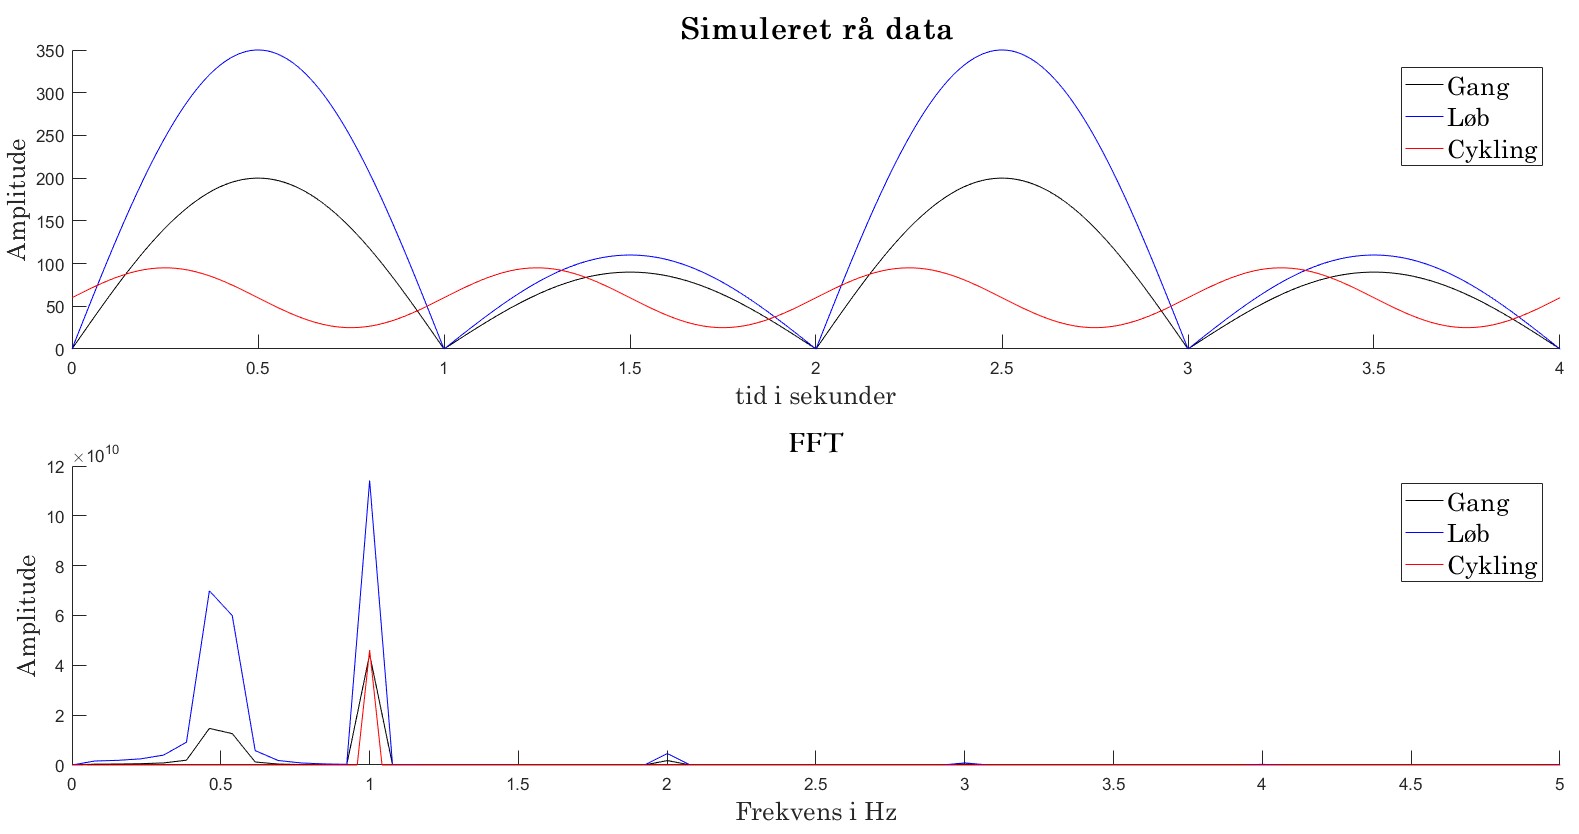
\includegraphics[scale=0.3]{figures/cDesign/gyro_behandling.png}
	\caption{På figuren ses øverst rå data fra pilotforsøget for gang, løb og cykling optaget med gyroskopets z-akse. Nederst ses frekvensdomænet for det nævnte data. Den sorte kurve viser data for gang, den grønne kurve viser data for løb og den røde kurve viser data for cykling.}
	\label{fig:gyro_behandling}
\end{figure}\vspace{-0.25cm}
\Figref{fig:gyro_behandling} viser, at signalets frekvenser og deres tilhørende magnituder kommer til udtryk. I andet trin findes frekvensværdien for den maksimale peak. Amplituden herfra bliver summeret i det tredje trin sammen med magnituderne for $\pm$1~Hz af den pågældende frekvens med maksimal peak. Derved fås en magnitudeværdi for maksimal peak værdi summeret med de to omkringliggende magnitudeværdier. Derudover summeres magnitudeværdierne for FFTen fra 1 til 20~Hz i det tredje trin, som herefter vil blive betegnet som hele FFTen. Resultatet heraf består af en magnitudeværdi for den maksimale peak med omkringliggende værdier, samt en magnitudeværdi for hele FFTen. Disse to summeringer benyttes til fjerde og sidste trin, som omregner hvor stor en procentdel den første summering med det højeste peak udgør i forhold til hele FFTen. Summeringen over den maksimale peak med omkringliggende værdier vil udgøre en stor procentdel af den samlede summering, når signaler fra cykling analyseres. Dette skyldes, at cykling afspejles som et sinussignal, hvoraf energien befinder sig omkring få frekvenser. Aktiviteterne gang og løb har ikke samme karakteristiske påvirkning af gyroskopet, når de behandles med overstående signalbehandling.

Data fra pilotforsøget er behandlet med ovenstående signalbehandling. Dette er gjort med henblik på fastsættelse af en tærskelværdi som adskiller cykling fra gang og løb. På den øverste graf på \figref{fig:gyro_behandling} ses de rå signaler fra gyroskopet for aktiviteterne gang, løb og cykling. Som det afspejles, er cykling tilnærmelsesvis som en sinussignal, hvorfor dennes energi er centreret omkring få frekvenser. Resultatet af signalbehandlingen ses på den nederste graf på \figref{fig:gyro_behandling}. Signalerne for gang, løb og cykling er behandlet med en FFT. På \figref{fig:gyro_behandling} ses det, at energien for gang og løb ikke centrerer sig omkring en enkelt frekvens, men om forskellige frekvenser. Denne spredning af energi kan benyttes til signalgenkendelse og adskillelse af aktiviteterne. 

Efter ovenstående signalbehandlingen implementeres signalgenkendelsen, som består af først at finde den maksimale magnitude og den tilhørende frekvens. Resultatet heraf er aktivitetens dominerende frekvens. Herefter summeres værdierne for den maksimale magnitude ved at summere intervallet $\pm$1~Hz omkring frekvens heraf. Hertil summeres også værdierne for FFTen fra 1 til 20~Hz. Afslutningsvist bestemmes hvor stor en procentdel summeringen for den maksimale magnitude udgør af summeringen for 1 til 20~Hz.\\ 
\begin{table}[H]
	\centering
	\begin{tabular}{cccc}
		\hline
		\rowcolor[HTML]{C0C0C0} 
		Forsøgsperson & \begin{tabular}[c]{@{}c@{}} Procentdel af totalen \\ for gang {[}\%{]} \end{tabular} & \begin{tabular}[c]{@{}c@{}} Procentdel af totalen \\ for løb {[}\%{]} \end{tabular} & \begin{tabular}[c]{@{}c@{}} Procentdel af totalen \\ for cykling {[}\%{]} \end{tabular} \\ \hline
		F1 & 41,0 & 38,6 & 85,5 \\ \hline	
		F2 & 48,5 & 51,5 & 91,9 \\ \hline	
		F3 & 35,9 & 42,8 & 85,0 \\ \hline
		F4 & 38,7 & 60,6 & 91,6 \\ \hline
	\end{tabular}
	\caption{I tabellen ses det, hvor stor en procentdel de største magnituder udgør af hele frekvensdomænet. Den største procentdel er at finde ved cykling.}
	\label{tab:individuel_procent}
\end{table}\vspace{-0.25cm}
Mængden af energi ved den maksimale magnitude er markant større for cykling i forhold til gang og løb, hvilket er illustreret i \tabref{tab:individuel_procent}. Dette resulterer i, at 85\% til 91,9\% af energien ligger $\pm$1~Hz omkring den fundne frekvens med den største magnitude. Procentfordelingen bliver ligeledes behandlet for gang og løb for at sikre, at disse ikke har samme spredning i frekvensområdet, hvormed en mulig tærskelværdi til detektering af cykling kan fastsættes. Resultatet heraf viser, at ved gang befinder energien omkring den fundne maksimale peak sig mellem 35,9\% til 48,5\% i forhold til det samlede frekvensspektrum. Ved løb befinder energien omkring den fundne frekvens sig mellem 38,6\% til 60,6\%. Denne forskel benyttes til at adskille cykling fra gang og løb ved at implementere et tærskelværdi på 70\%. Summeringen af magnituden omkring den største magnitude skal dermed udgøre mindst 70\% for at blive klassificeret som cykling. 
\begin{figure}[H]
	\centering
	\includegraphics[scale=0.5]{figures/cDesign/algoritme_cykling2.png}
	\caption{På figuren ses et flowchart over de overordnede funktioner for algoritmen til detektering af cykling.}
	\label{fig:algoritme_cykling}
\end{figure}\vspace{-0.25cm}
\Figref{fig:algoritme_cykling} repræsenterer algoritmen for detektering af cykling. Data fra gyroskopet sendes til MATLAB, hvorefter overstående signalbehandling fortages. Hvis resultatet heraf er over 70\%, kategoriseres det behandlede data som værende cykling, hvorefter fire sekunders cykling adderes til varigheden for aktiviteten. Hvis signalet ikke overstiger 70\%, starter algoritmen forfra.

\subsection{Implementering}
Implementeringen af algoritmen for detektering af cykling tager udgangspunkt i data fra pilotforsøget og de designmæssige aspekter, som er beskrevet i \secref{design_cykling}. Algoritmen er designet og implementeret, som det ses på \figref{fig:basic_cykling}.
\begin{figure}[H]
	\centering
	\includegraphics[scale=0.4]{figures/cDesign/Algoritme_cykling_basic.png}
	\caption{På figuren ses et flowchart over den implementerede algoritme, i henholdsvis MATLAB og C kode. Algoritmen omhandler detektering af cykling. Den markerede kasse, signalbehandling, indeholder yderligere kodning, som forklares uddybende efterfølgende.}
	\label{fig:basic_cykling}
\end{figure}\vspace{-0.25cm}
Algoritmen henter low og high byte fra gyroskopets output, hvorefter hver enkelt sample videresendes til MATLAB. Yderligere fremgår signalbehandlingen på \figref{fig:matlab_cykling}.
\begin{figure}[H]
	\centering
	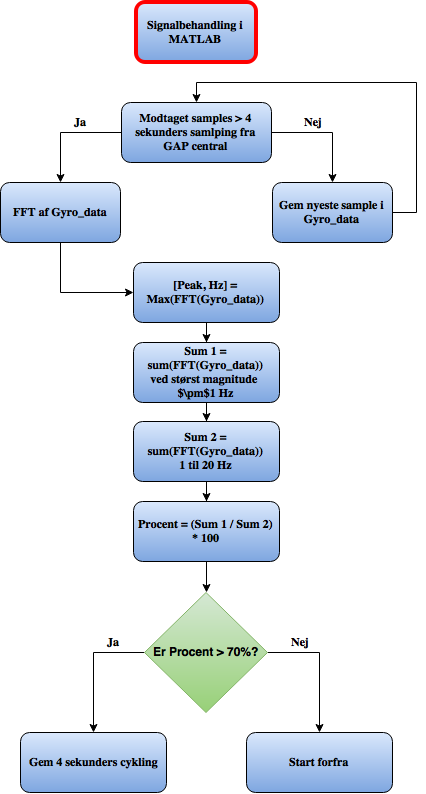
\includegraphics[scale=0.4]{figures/cDesign/algoritme_matlab_cykling.png}
	\caption{På figuren ses et flowchart over algoritmens signalbehandling, udført i MATLAB. Koden benytter fire sekunders sampling, hvis frekvensdomæne analyseres. Derefter foretages en vurdering af de maksimale magnituder i forhold til resten af frekvensdomænet.}
	\label{fig:matlab_cykling}
\end{figure}\vspace{-0.25cm}
I MATLAB gemmes 4~sekunders data i et array, hvorefter signalbehandlingen påbegyndes. Denne indbefatter en FFT behandling af signalet, hvorefter maksimal magnitude værdi detekteres. Herefter sammenlignes summeringen for maksimal magnitude med den samlede summering. Resultatet heraf er en procentværdi for det modtagne data. Denne værdi undersøges for at være over eller under tærskelværdien. Hvis resultatet er over 70\% summeres fire sekunder til den totale varighed for cykling i GUI. Derefter startes algoritmen forfra. Hvis cyklingen ikke detekteres, starter algoritmen ligeledes forfra. 

\subsection{Test}
Algoritmens funktioner testes individuelt og samlet. Dette gøres for at be- eller afkræfte om algoritmen lever op til de opstillede krav i \secref{krav_algoritme}, som lyder at algoritmen skal:
\begin{itemize}
	\item Behandle data fra gyroskopet, således frekvensindholdet fra signalet fremstår.
	\item Være i stand til at detektere cykling ved procentfordeling af frekvensindhold. Det accepteres ikke, at systemet ikke kan detektere og adskille cykling fra gang og løb.
\end{itemize}

Først testes algoritmens fire sekunders time counter. Måden hvorpå denne testes er ved at plotte resultatet af MATLABs time counter. Det undersøges hvorvidt time counteren tæller op til fire sekunder, når der er modtaget fire sekunders data. Hvis dette er tilfældet skal time counteren nulstilles. Dette testes ved at indsende 1904~samples, hvilket svarer til fire sekunder med en samplingsfrekvens på 476.  
\begin{figure}[H]
	\centering
	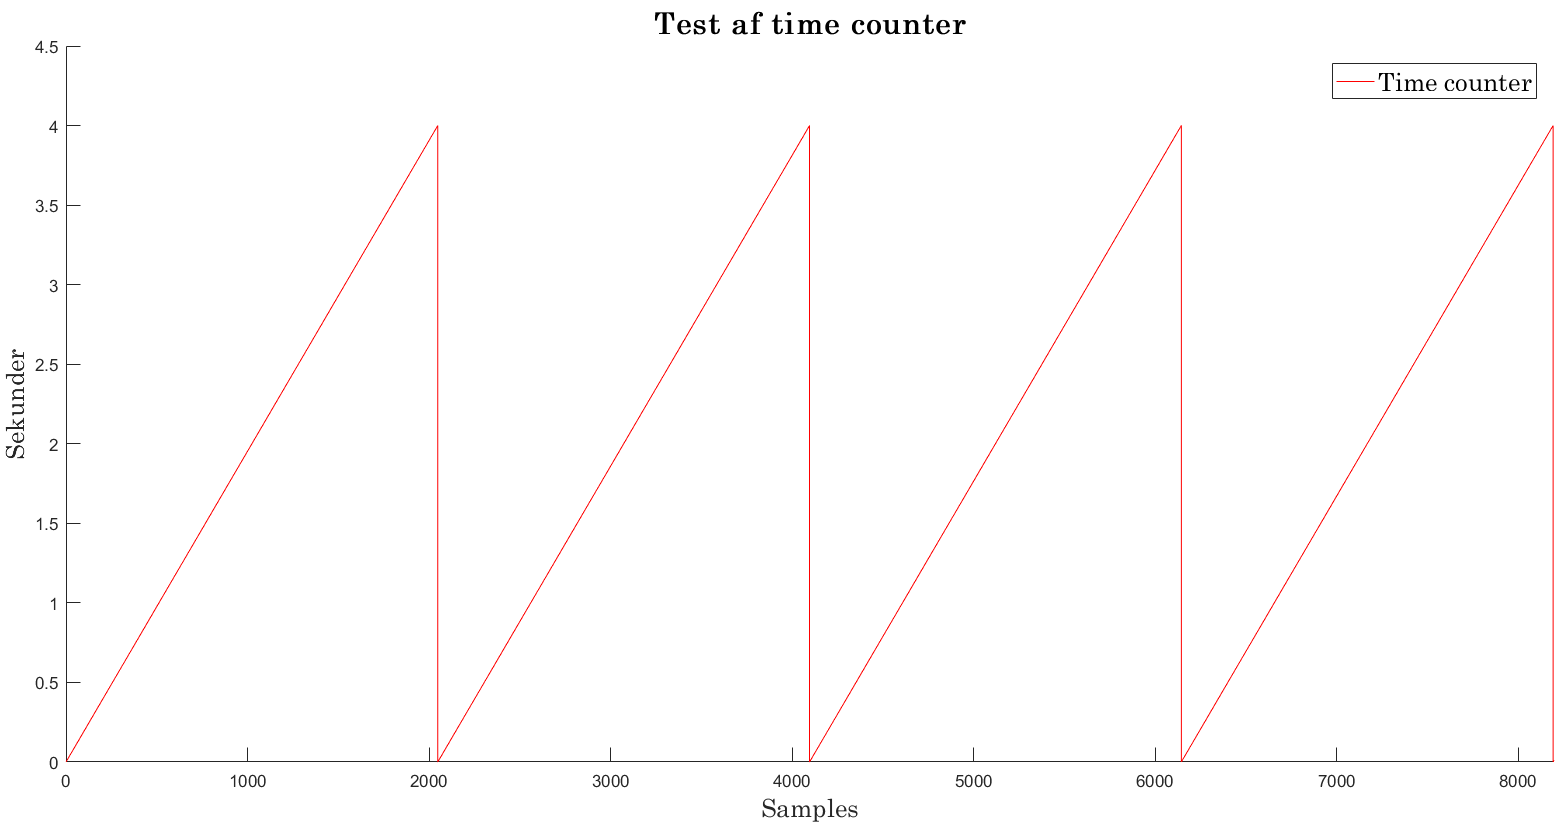
\includegraphics[width=.7\textwidth]{figures/cDesign/sim_counter.png}
	\caption{På figuren ses algoritmens time counter plottet med rød. Det ses, at time counteren tæller op til fire sekunder og derefter nulstilles og starter forfra.}
	\label{fig:sim_count}
\end{figure}\vspace{-.25cm}
Time counteren tæller til fire sekunder bestående af 1904 samples, hvorefter denne nulstilles.\\
Den anden test, omhandler hvorledes FFTen stemmer overens med forventningerne hertil. Der indsendes et sinussignal som skal repræsentere cykling med en frekvens på 1~Hz. For henholdsvis gang og løb indsendes der et absolut sinussignal med varierende amplitude. Forventningen af resultatet bør medføre at energien af det simulerede signal vedrørende cykling er fordelt omkring 1 Hz, og de resterende er spredt over flere frekvenser. Resultatet af denne test ses illustreret på \figref{fig:sim_gyro}, hvor de simulerede rå signaler ses på øverste graf, mens FFTen for signalerne ses på nederste graf.
\begin{figure}[H]
	\centering
	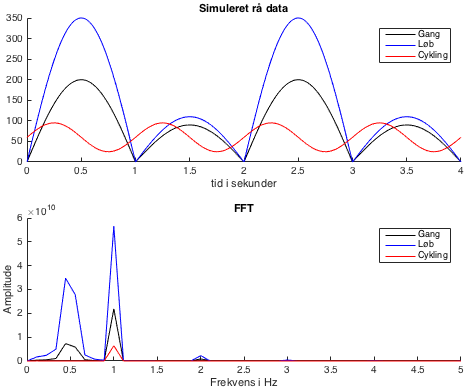
\includegraphics[width=.75\textwidth]{figures/cDesign/sim_gyro.png}
	\caption{På figurens øverste graf ses de simulerede inputsignaler for gang, løb og cykling. Den nederste graf viser frekvensdomæneanalysen af de pågældende signaler.}
	\label{fig:sim_gyro}
\end{figure}\vspace{-.25cm}
Som forventet ses det på \figref{fig:sim_gyro}, at FFTen for det simulerede signal af cykling centreres omkring 1~Hz, mens signalerne for gang og løb centreres omkring 0,5~Hz, 1~Hz og 2~Hz. Da det er forskelligt, om de tre simulerede signaler centreres om én eller flere frekvenser forventes det, at spredningen af signalets energi varierer for de tre aktiviteter, hvilket den tredje test vil undersøge. Heraf forventes det at spredningen af energien ved cykling er markant mindre end spredningen af energi ved gang og løb. Som beskrevet i \secref{design_cykling} forventes minimum 70\% af energien ved cykling at være indenfor $\pm$1~Hz omkring den maksimale peak af FFTen, hvorimod det ved gang og løb forventes at være markant mindre. 
\begin{table}[H]
\centering
\begin{tabular}{ccc}
	\hline
	\cellcolor[HTML]{C0C0C0}\begin{tabular}[c]{@{}c@{}}Procentdel af totalen \\ for gang [\%]\end{tabular} & \cellcolor[HTML]{C0C0C0}\begin{tabular}[c]{@{}c@{}}Procentdel af totalen \\ for løb [\%]\end{tabular} & \cellcolor[HTML]{C0C0C0}\begin{tabular}[c]{@{}c@{}}Procentdel af totalen \\ for cykling [\%]\end{tabular} \\ \hline
	56,85 & 42,46 & 99,28 \\ \hline
\end{tabular}\vspace{-.25cm}
	\caption{I tabellen ses hvor mange procent den maksimale frekvensmagnitude udgør af 1-20~Hz ved simuleringerne for gang, løb og cykling.}
	\label{tab:sim_procent}
\end{table}\vspace{-.25cm}
Som det fremgår af \tabref{tab:sim_procent} udgør procentdelen af totalen vedrørende cykling markant mere af den samlede energi end ved gang og løb. Dette opfylder kravet angående, at algoritmen bør kunne detektere og adskille cykling fra gang og løb som resultat af procentfordelingen af frekvensdomænet. %Dette er tilfældet, hvis data afspejles som det simulerede signal samt data fra pilotforsøget.

%Afslutningsvist testes algoritmens funktionalitet omhandlende dets resultat ved behandling af et signal, som overskrider tærskelværdien på 70\%. Det undersøges, om der gemmes 4 sekunder til varigheden for udført cykling, som resultat af hver detektering.
%\begin{figure}[H]
%	\centering
%	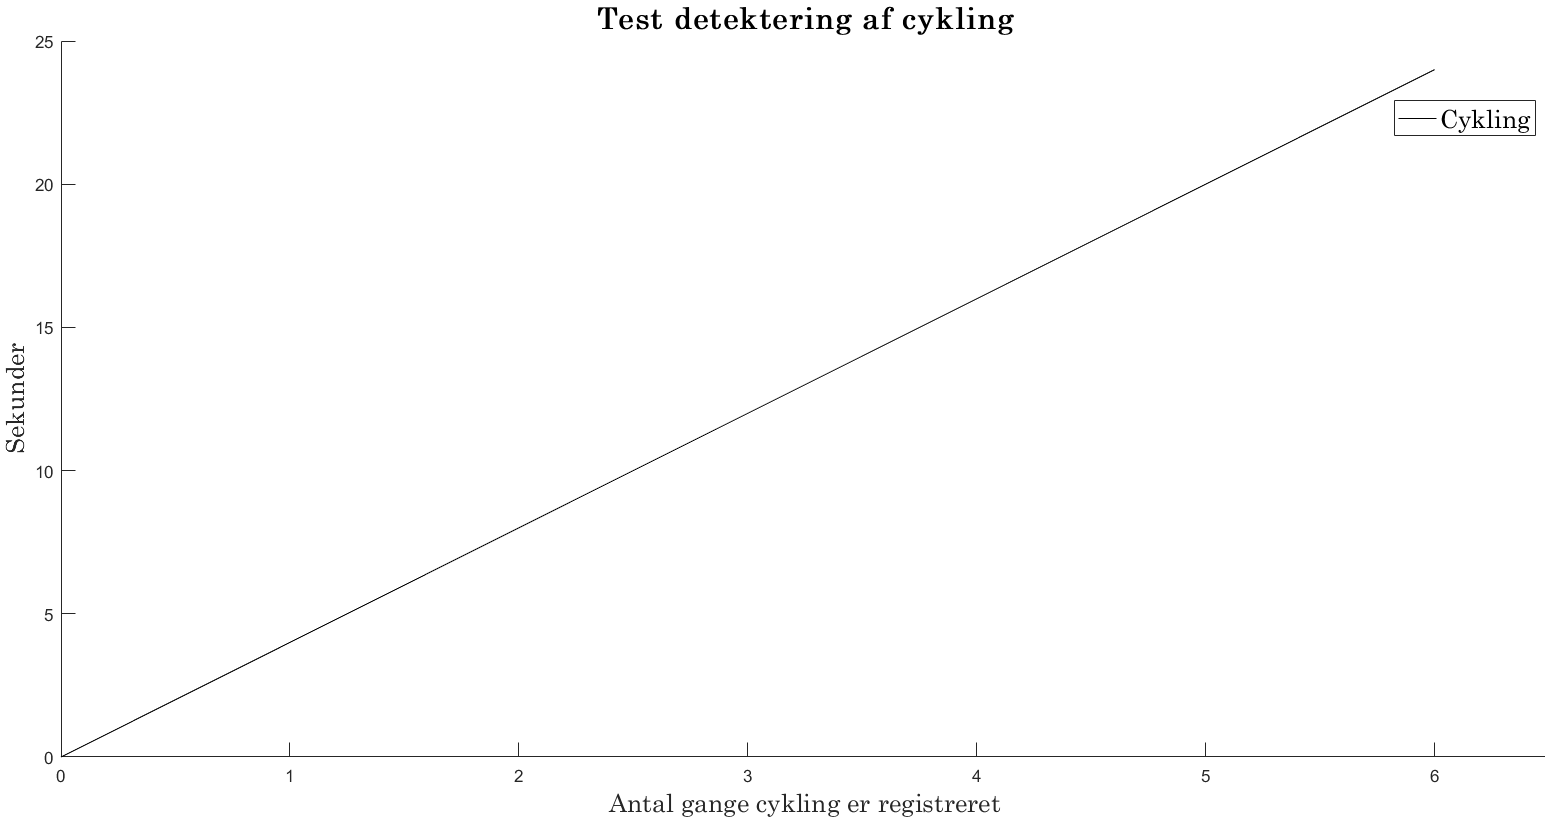
\includegraphics[width=.7\textwidth]{figures/cDesign/sim_n_c.png}
%	\caption{På figuren ses en lineær graf som viser antallet af sekunder der registreret cykling, som funktion af antal gange at aktiviteten er detekteret. Hver detektering af cykling giver et output på 4 sekunder for aktiviteten.}
%	\label{fig:sim_n_cykling}
%\end{figure}\vspace{-.25cm}
%Disse værdier vil blive brugt i GUI til at repræsentere brugerens cyklingsaktivitet. Mens de signaler, som ikke opfattes som cykling, vil blive kasseret, da gang og løb repræsenteres ved hjælp af accelerometerdata som beskrevet i \secref{sec:algogangloeb}. 